\section{Results}
\label{sec:results}

\subsection{The Inverted Tell: AI Deception Reverses Human Patterns}
\label{sec:inverted_tell}

Our central finding is that AI deception systematically inverts three of four established human deception signals. Table~\ref{tab:inversion_summary} summarizes the comparison and Figure~\ref{fig:inverted_tell} visualizes the per-model shifts.

\begin{table}[t]
\caption{Summary of deception signal directions: human liars (from meta-analyses) vs.\ AI liars (our data, consistent across all 8 models unless noted). ``Inverted'' means the AI pattern is opposite to the human pattern.}
\label{tab:inversion_summary}
\centering
\small
\begin{tabular}{lccc}
\toprule
\textbf{Feature} & \textbf{Human Liars} & \textbf{AI Liars} & \textbf{Alignment} \\
\midrule
First-person pronouns & Decrease & Increase (all 8) & Inverted \\
Message length & Decrease & Increase (all 8) & Inverted \\
Hedging language & Varies & Increase (7 of 8) & Partially inverted \\
Negative sentiment & Increase & Increase (5 of 8) & Same direction \\
\bottomrule
\end{tabular}
\end{table}

\paragraph{First-person pronouns.} Human deception research consistently finds that liars use fewer first-person singular pronouns, interpreted as psychological distancing from the lie \citep{newman2003lying}. In our data, \emph{every} model shows the opposite: werewolves use \emph{more} ``I/me/my'' than villagers, with increases ranging from +0.55 percentage points (Grok 4.1) to +1.02 pp (Gemini 3 Pro). Table~\ref{tab:pronouns} presents the full results.

\begin{table}[t]
\caption{First-person pronoun usage (I/me/my/mine) as percentage of total words, by role. All 8 models show increased self-reference when deceiving.}
\label{tab:pronouns}
\centering
\small
\begin{tabular}{lrrr}
\toprule
\textbf{Model} & \textbf{As WW (\%)} & \textbf{As Villager (\%)} & \textbf{$\Delta$ (pp)} \\
\midrule
Gemini 3 Pro Preview & 4.40 & 3.38 & +1.02 \\
Gemini 3 Flash Preview & 3.96 & 3.22 & +0.75 \\
GPT-5.2 & 3.43 & 2.77 & +0.66 \\
Claude Opus 4.5 & 4.36 & 3.70 & +0.66 \\
Claude Sonnet 4.5 & 4.08 & 3.22 & +0.85 \\
Grok 4.1 Fast Reasoning & 2.57 & 2.02 & +0.55 \\
Grok 4 & 4.09 & 3.14 & +0.96 \\
GPT-5 mini & 4.06 & 3.40 & +0.66 \\
\bottomrule
\end{tabular}
\end{table}

This inversion is remarkably consistent: 8 out of 8 models, spanning four different providers and a wide range of architectures and training methodologies, all show the same reversal (Figure~\ref{fig:pronoun_comparison}). We discuss possible explanations in Section~\ref{sec:discussion}.

\begin{figure}[t]
\centering
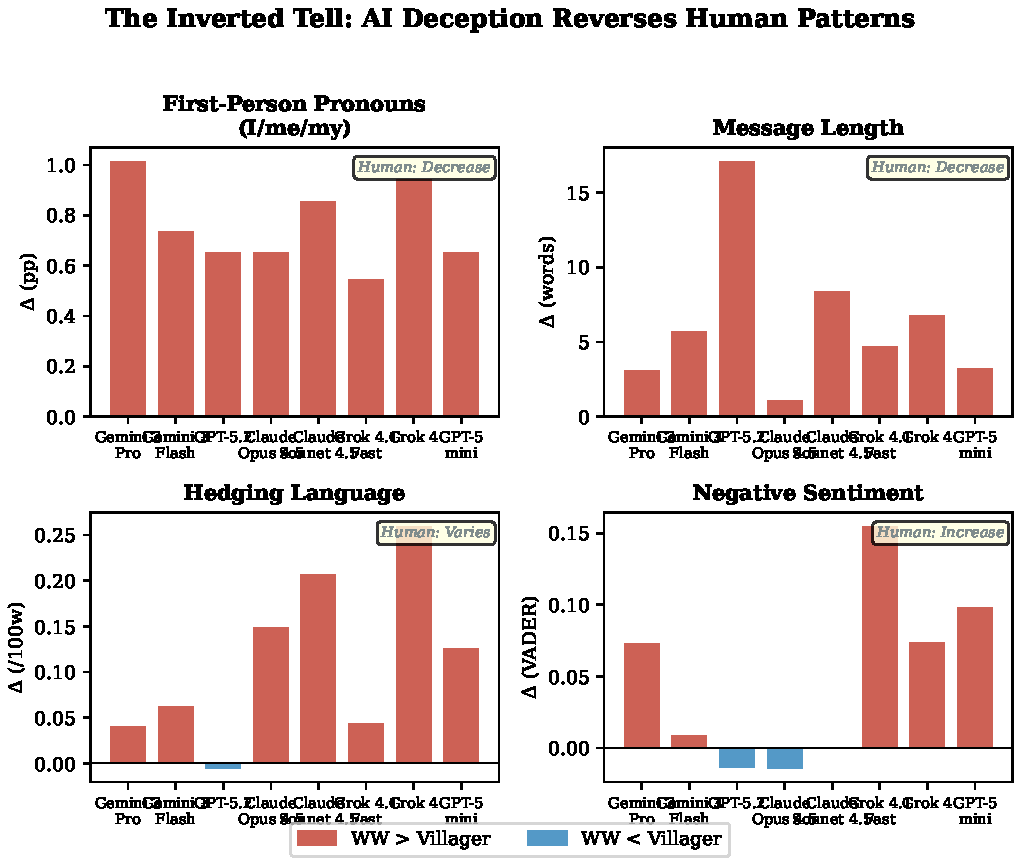
\includegraphics[width=\textwidth]{figures/fig1_inverted_tell.pdf}
\caption{The Inverted Tell across all 8 models. Red bars indicate the AI werewolf value exceeds the villager value; blue indicates the reverse. Models are ordered by werewolf win rate (left = best). Three of four features show consistent inversion of human deception patterns.}
\label{fig:inverted_tell}
\end{figure}

\begin{figure}[t]
\centering
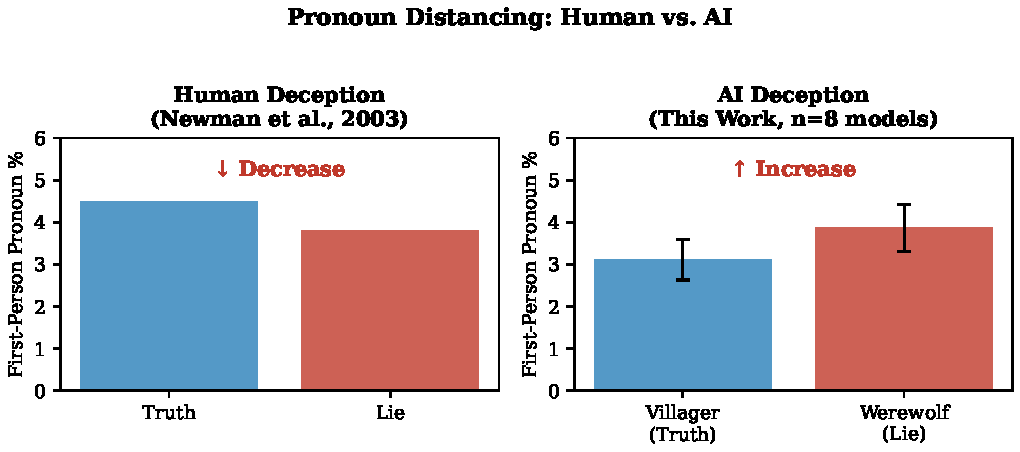
\includegraphics[width=0.85\textwidth]{figures/fig4_pronoun_comparison.pdf}
\caption{First-person pronoun usage in deception: human liars decrease self-reference (left, schematic from \citet{newman2003lying}), while AI liars increase it (right, averaged across 8 models with standard deviation bars).}
\label{fig:pronoun_comparison}
\end{figure}

\paragraph{Message length.} Human liars tend to produce shorter, less detailed statements \citep{depaulo2003cues}. Every AI model in our dataset produces \emph{longer} messages as werewolf, with increases ranging from +1.2 words (Claude Opus 4.5) to +17.2 words (GPT-5.2, a 21\% increase). Table~\ref{tab:length} shows the full results.

\begin{table}[t]
\caption{Average message length (words) by role. All 8 models write longer messages when deceiving.}
\label{tab:length}
\centering
\small
\begin{tabular}{lrrrr}
\toprule
\textbf{Model} & \textbf{WW Msgs} & \textbf{WW Avg} & \textbf{Vill Avg} & \textbf{$\Delta$ Words} \\
\midrule
Gemini 3 Pro & 34,537 & 70.0 & 66.8 & +3.1 \\
Gemini 3 Flash & 32,483 & 74.5 & 68.7 & +5.9 \\
GPT-5.2 & 30,777 & 100.0 & 82.8 & +17.2 \\
Claude Opus 4.5 & 32,760 & 116.3 & 115.1 & +1.2 \\
Claude Sonnet 4.5 & 33,252 & 100.9 & 92.4 & +8.5 \\
Grok 4.1 Fast & 30,094 & 43.6 & 38.8 & +4.8 \\
Grok 4 & 28,175 & 56.3 & 49.4 & +6.8 \\
GPT-5 mini & 24,216 & 69.9 & 66.6 & +3.3 \\
\bottomrule
\end{tabular}
\end{table}

\paragraph{Hedging and certainty.} Seven of eight models show increased hedging language as werewolf, with Grok 4 showing the largest increase (+0.260 per 100 words). Simultaneously, all eight models show \emph{decreased} certainty language as werewolf, with Grok 4.1 showing the largest drop ($-0.302$ per 100 words). The one exception to the hedging pattern is GPT-5.2, which shows a negligible decrease ($-0.008$). This pattern---more hedging, less certainty---is the opposite of what would be expected if AI liars, like human liars, showed reduced cognitive complexity.

\paragraph{Sentiment.} Five of eight models show more negative sentiment as werewolf, consistent with the human deception finding of increased negative affect. However, the effect is inconsistent: Claude Opus 4.5, GPT-5.2, and Claude Sonnet 4.5 show slightly \emph{more positive} sentiment as werewolf. Sentiment is the one dimension where AI and human deception patterns partially align.

\subsection{The Best Liars Change Least}
\label{sec:best_liars}

We next ask: among the eight models, which features predict successful deception? Table~\ref{tab:correlations} shows Spearman rank correlations between linguistic shift magnitudes and werewolf win rate.

\begin{table}[t]
\caption{Spearman rank correlations between linguistic feature shifts ($\Delta$) and werewolf win rate ($n = 8$ models). Negative correlations indicate that \emph{smaller} shifts predict better performance.}
\label{tab:correlations}
\centering
\small
\begin{tabular}{lr}
\toprule
\textbf{Feature Shift} & \textbf{$\rho$ with WW Win Rate} \\
\midrule
Hedge word increase & $-0.64$ \\
Deception gap (sentiment) & $-0.36$ \\
Fake Seer claim rate & $-0.26$ \\
Message length increase & $+0.00$ \\
\bottomrule
\end{tabular}
\end{table}

The strongest predictor is hedging increase ($\rho = -0.64$): models that hedge more as werewolf perform \emph{worse} (Figure~\ref{fig:best_liars}). The deception gap ($\rho = -0.36$) and fake Seer claim rate ($\rho = -0.26$) show similar patterns---more overt deception signals correlate with worse outcomes. We note that with $n = 8$, none of these individual correlations reach conventional significance thresholds ($|\rho| > 0.74$ required for $p < 0.05$); we report them as descriptive effect sizes, with the converging pattern across multiple features providing the primary evidence.

This result crystallizes in the contrast between the best and worst werewolves:
\begin{itemize}
    \item \textbf{Gemini 3 Pro} (44.6\% WW win rate): smallest hedging increase (+0.042), lowest fake Seer rate (7.82\%), and a \emph{negative} deception gap ($-0.037$, meaning its public messages are actually slightly more negative than its private reasoning).
    \item \textbf{GPT-5 mini} (13.6\% WW win rate): large hedging increase (+0.128), high early accusation rate (61.3\% on Day 1), and the lowest overall survival rate (31.5\%).
\end{itemize}

\begin{figure}[t]
\centering
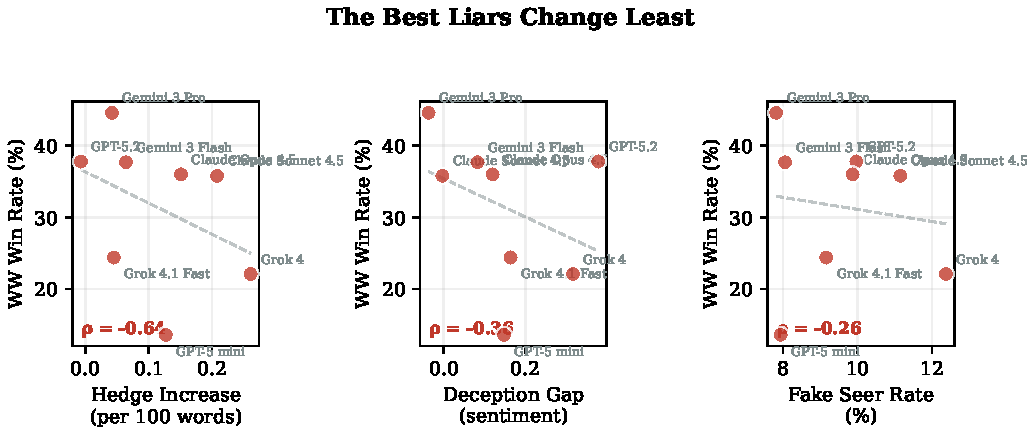
\includegraphics[width=\textwidth]{figures/fig2_best_liars.pdf}
\caption{Behavioral shift magnitude vs.\ werewolf win rate. Larger shifts (more hedging, bigger deception gap, more fake claims) correlate with \emph{worse} performance. The best deceivers change their behavior the least.}
\label{fig:best_liars}
\end{figure}

The implication is clear: successful AI deception is characterized by \emph{behavioral consistency}, not active manipulation. The best AI liars are those whose werewolf behavior is most similar to their villager behavior---making them hardest to distinguish through behavioral analysis.

\subsection{Model Performance Hierarchy}
\label{sec:performance}

Table~\ref{tab:performance} and Figure~\ref{fig:performance} present the complete model performance breakdown. The meta is heavily villager-favored (68.4\% village win rate), making werewolf performance the primary differentiator between models.

\begin{figure}[t]
\centering
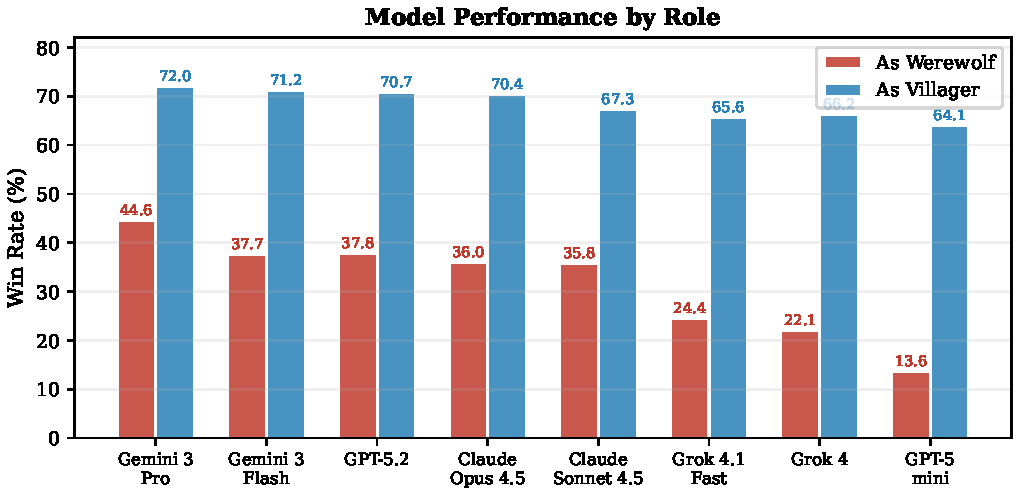
\includegraphics[width=0.9\textwidth]{figures/fig3_performance.pdf}
\caption{Win rates by role across all 8 models. Villager win rates cluster tightly (64--72\%), while werewolf win rates span a 31-point range (14--45\%), indicating that deception ability is the primary differentiator.}
\label{fig:performance}
\end{figure}

\begin{table}[t]
\caption{Model performance across roles. WW = Werewolf. Win rate = fraction of games where the model's team won.}
\label{tab:performance}
\centering
\small
\begin{tabular}{lrrrr}
\toprule
\textbf{Model} & \textbf{Games} & \textbf{Overall} & \textbf{As WW} & \textbf{As Villager} \\
\midrule
Gemini 3 Pro & 31,619 & 65.0\% & 44.6\% & 72.0\% \\
Gemini 3 Flash & 31,197 & 63.0\% & 37.7\% & 71.2\% \\
GPT-5.2 & 31,423 & 62.6\% & 37.8\% & 70.7\% \\
Claude Opus 4.5 & 31,212 & 61.8\% & 36.0\% & 70.4\% \\
Claude Sonnet 4.5 & 31,574 & 59.4\% & 35.8\% & 67.3\% \\
Grok 4.1 Fast & 31,645 & 55.3\% & 24.4\% & 65.6\% \\
Grok 4 & 31,667 & 55.2\% & 22.1\% & 66.2\% \\
GPT-5 mini & 31,495 & 51.6\% & 13.6\% & 64.1\% \\
\bottomrule
\end{tabular}
\end{table}

Villager win rates cluster tightly (64.1\%--72.0\%), while werewolf win rates span a 31-point range (13.6\%--44.6\%). This suggests that the village role primarily requires baseline competence (follow evidence, vote with the group), while the werewolf role---which requires active deception---is where model capability differences manifest most strongly.

\subsection{Strategic Findings}
\label{sec:strategic}

\paragraph{Seer impact.} The Seer is the most impactful role. When the Seer successfully identifies a werewolf, the village wins 79.4\% of games; when the Seer fails to find any werewolf, the village win rate drops to 41.7\%---a 37.7 percentage point swing.

\paragraph{Night 0 targeting.} Killing the Seer on Night 0 is the single most effective werewolf strategy, yielding a 48.2\% werewolf win rate compared to 27.7\% when a villager is killed and 30.0\% when the Doctor is killed. However, werewolves kill the Seer on Night 0 only 19.9\% of the time (close to the 12.5\% random baseline for an 8-player game with 1 Seer, suggesting limited strategic targeting).

\paragraph{Werewolf duos.} Same-model werewolf pairs dramatically outperform mixed pairs. Gemini 3 Pro duos win 52.1\% of games---the only duo exceeding 50\%---compared to 31.7\% for mixed-model duos. At the other extreme, GPT-5 mini duos win only 3.4\% of games. This suggests that implicit coordination between same-model agents (shared reasoning patterns, compatible strategies) provides a substantial advantage.

\paragraph{Bus rate.} Gemini 3 Pro has the highest bus rate (17.5\%), meaning it most frequently votes against its own werewolf partner. This counterintuitive strategy---sacrificing your ally to maintain cover---correlates with higher werewolf win rates, consistent with advanced Mafia strategy.

\paragraph{Speaking order.} The last speaker on Day 1 wins 10--16\% more often than the first speaker across all models, confirming the last-speaker advantage observed in human Mafia games \citep{costa2025minimafia}. The last speaker benefits from observing all prior statements before committing to a position.

\subsection{The Deception Gap: What Models Think vs.\ What They Say}
\label{sec:deception_gap}

The availability of private reasoning enables a unique analysis of the divergence between internal state and public presentation. Table~\ref{tab:deception_gap} shows the deception gap for each model.

\begin{table}[t]
\caption{The deception gap: difference between public message sentiment and private reasoning sentiment for werewolf players. A positive gap indicates ``fake nice'' behavior.}
\label{tab:deception_gap}
\centering
\small
\begin{tabular}{lrrr}
\toprule
\textbf{Model} & \textbf{Avg Reasoning} & \textbf{Avg Message} & \textbf{Gap} \\
\midrule
GPT-5.2 & $-0.073$ & $+0.306$ & $+0.379$ \\
Grok 4 & $-0.283$ & $+0.034$ & $+0.317$ \\
Grok 4.1 Fast & $-0.229$ & $-0.066$ & $+0.164$ \\
GPT-5 mini & $-0.069$ & $+0.080$ & $+0.148$ \\
Claude Opus 4.5 & $+0.128$ & $+0.249$ & $+0.120$ \\
Gemini 3 Flash & $+0.166$ & $+0.249$ & $+0.083$ \\
Claude Sonnet 4.5 & $+0.150$ & $+0.147$ & $-0.003$ \\
Gemini 3 Pro & $+0.118$ & $+0.082$ & $-0.037$ \\
\bottomrule
\end{tabular}
\end{table}

GPT-5.2 has the largest deception gap (+0.379): internally negative ($-0.073$) but publicly positive ($+0.306$). Notably, the two most successful werewolves---Gemini 3 Pro and GPT-5.2---sit at opposite ends of this spectrum: Gemini 3 Pro has a \emph{negative} gap (it is actually slightly more negative publicly than privately), while GPT-5.2 has the largest positive gap. This suggests that the deception gap alone does not determine success; rather, it is the overall \emph{consistency} of behavior across roles that matters.
